\section{Experiments and results}

\subsection{Experimental setup}

All experiments ran locally on one laptop with an NVIDIA GeForce RTX 3060 Laptop GPU (6\,GB) under Windows~11, with Python \VerPython{}, NumPy \VerNumpy{}, scikit-learn \VerSklearn{}, SciPy \VerScipy{}, PyTorch \VerTorch{}, torchvision \VerTorchvision{} and OpenCV \VerOpencv{}. Feature extraction for the 39 trials took about three minutes, dominated by optical flow, and the evaluation of all models including the bootstrap and permutation analyses took under two minutes. Every randomised step uses seed 0. Before the full run, the feature extractors were checked on a single trial (B001), which confirmed the frame counts, the alignment of the 5635 kinematic samples with the 5640 video frames, and the official fold membership. The full pipeline was then run once, and every number in this report is read from its output file.

\subsection{Quantitative results}

Table~\ref{tab:main} and Figure~\ref{fig:results} give the results of all models. The majority-class baseline always predicts novice, which is right for 19 of 39 trials (accuracy \AccMZero{}) and gives macro-F1 \FMZero{}, because the intermediate and expert classes receive F1 of zero. The kinematics-only baseline K-simple (M1) reaches macro-F1 \FMOne{} (95\% interval \LoMOne{} to \HiMOne{}) and accuracy \AccMOne{}. Its paired difference from the majority class is \DOneZero{} with interval \DLoOneZero{} to \DHiOneZero{}, which excludes zero, and the exact permutation test gives $p = \PMOne{}$. The first pre-declared comparison is therefore supported: simple trial statistics carry skill information that transfers to unseen surgeons, although the lower end of the interval is close to the majority level.

\begin{table}[htbp]
\centering
\small
\caption{Leave-one-user-out results on JIGSAWS Suturing (39 trials, 8 surgeons). Macro-F1, accuracy and per-class F1 are computed over the pooled out-of-fold predictions. The interval is the 2.5th to 97.5th percentile of 2000 user-level bootstrap resamples; $p$ is the exact user-level permutation $p$-value over all 420 label assignments. Bold rows are the kinematic baseline, the primary multimodal model and the focused improvement.}
\label{tab:main}
\begin{tabular}{@{}l l c c c c c c@{}}
\toprule
Model & ID & Macro-F1 [95\% CI] & Acc. & F1$_\mathrm{N}$ & F1$_\mathrm{I}$ & F1$_\mathrm{E}$ & $p$ \\
\midrule
\multicolumn{8}{@{}l}{\textit{Required experiment}} \\
\quad Majority class & M0 & 0.218 [0.074, 0.310] & 0.487 & 0.66 & 0.00 & 0.00 & 1.000 \\
\quad K-simple & M1 & \textbf{0.515} [0.272, 0.618] & 0.615 & 0.75 & 0.64 & 0.15 & 0.033 \\
\quad V-appear & M2a & 0.345 [0.125, 0.496] & 0.436 & 0.72 & 0.00 & 0.32 & 0.455 \\
\quad V-dyn & M2b & 0.371 [0.222, 0.467] & 0.487 & 0.75 & 0.36 & 0.00 & 0.348 \\
\quad V-flow & M2c & 0.420 [0.178, 0.576] & 0.513 & 0.67 & 0.59 & 0.00 & 0.240 \\
\quad K-simple + V-dyn, late (primary) & M3 & \textbf{0.443} [0.247, 0.568] & 0.538 & 0.75 & 0.45 & 0.12 & 0.188 \\
\quad K-simple + V-appear, late & M3b & 0.450 [0.253, 0.567] & 0.538 & 0.72 & 0.50 & 0.13 & 0.133 \\
\quad K-simple + V-flow, late & M3c & 0.481 [0.236, 0.596] & 0.615 & 0.75 & 0.69 & 0.00 & 0.062 \\
\quad K-simple + V-dyn, early & M3d & 0.461 [0.242, 0.564] & 0.615 & 0.74 & 0.64 & 0.00 & 0.036 \\
\addlinespace[2pt]
\multicolumn{8}{@{}l}{\textit{Focused improvement}} \\
\quad K-simple + K-texture & M4 & \textbf{0.520} [0.273, 0.619] & 0.615 & 0.75 & 0.67 & 0.14 & 0.074 \\
\quad (K-simple + K-texture) + V-dyn, late & M5 & 0.440 [0.259, 0.526] & 0.538 & 0.73 & 0.45 & 0.13 & 0.157 \\
\addlinespace[2pt]
\multicolumn{8}{@{}l}{\textit{Controls}} \\
\quad Duration only & C1 & 0.375 [0.275, 0.482] & 0.487 & 0.82 & 0.20 & 0.11 & 0.367 \\
\quad K-simple, residualised on log duration & C2 & 0.342 [0.167, 0.475] & 0.385 & 0.47 & 0.43 & 0.12 & 0.445 \\
\quad K-simple + K-texture, residualised & C2t & 0.344 [0.132, 0.509] & 0.385 & 0.38 & 0.53 & 0.12 & 0.371 \\
\bottomrule
\end{tabular}

\end{table}

None of the video blocks alone is distinguishable from chance. V-appear, V-dyn and V-flow reach macro-F1 of \FMTwoA{}, \FMTwoB{} and \FMTwoC{}, with permutation $p$-values of \PMTwoA{}, \PMTwoB{} and \PMTwoC{}. Adding video to kinematics did not help. The primary multimodal model (M3, late fusion of K-simple and V-dyn) reaches \FMThree{}, and its difference from K-simple is \DThreeOne{} (interval \DLoThreeOne{} to \DHiThreeOne{}). The interval includes zero, so the second pre-declared comparison is not distinguishable at this sample size, but the point estimate is negative, and every other fusion variant also scored below K-simple alone: \FMThreeB{} with V-appear, \FMThreeC{} with V-flow and \FMThreeD{} for early fusion with V-dyn (Figure~\ref{fig:results}b). The focused improvement (M4) adds the motion-texture block and reaches \FMFour{}. The difference from K-simple, \DFourOne{} (interval \DLoFourOne{} to \DHiFourOne{}), is negligible, so the third pre-declared comparison is not supported either. Combining the improved kinematic model with V-dyn (M5) gives \FMFive{}, again below its kinematic part.

\begin{figure}[htbp]
\centering
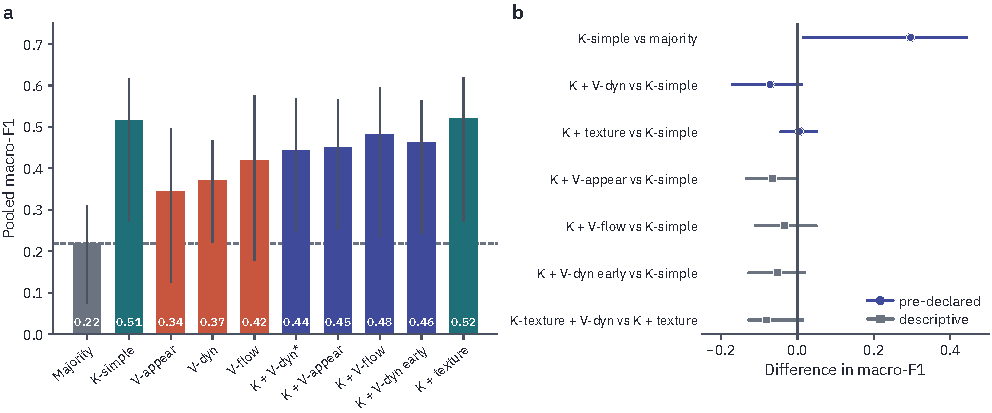
\includegraphics{fig3_results.pdf}
\caption{(a) Pooled macro-F1 of the majority class, the kinematic models (teal), the video-only models (red) and the fusion models (blue). Error bars are 95\% user-level bootstrap intervals; the dashed line is the majority-class score; * marks the pre-declared primary multimodal model. (b) Paired differences in macro-F1 with 95\% user-level bootstrap intervals. Circles are the three comparisons declared before the experiment; squares are descriptive comparisons.}
\label{fig:results}
\end{figure}

For comparison with the literature, \citet{zia2018rmis} report 88.2\% accuracy for Suturing under LOUO with approximate-entropy features. That figure is not directly comparable with ours. With 39 pooled predictions, accuracy moves in steps of 2.56 percentage points and 88.2\% is not attainable, so the published evaluation must have used a different trial set or a different aggregation, and it reports accuracy rather than macro-F1. The near-perfect results reported for deep networks on JIGSAWS mostly use LOSO, in which the test surgeon contributes training trials \citep{fawaz2018cnn, funke2019video}. Our bootstrap intervals, which are between about 0.25 and 0.4 wide in macro-F1, illustrate how little eight surgeons can resolve \citep{varoquaux2018cv}: a single surgeon changing class can move macro-F1 by more than 0.1.

\subsection{Analysis of successes and failures}

Figure~\ref{fig:confusion} shows where the errors occur. All three kinematic and multimodal models recognise novices well (F1 \FNMOne{} for K-simple) and intermediates moderately (F1 \FIMOne{}), but they almost never recognise experts (F1 \FEMOne{}). Of the ten expert trials, K-simple labels five as novice, four as intermediate and one as expert. Figure~\ref{fig:users} breaks this down by surgeon. The novices B and G and the intermediates C and F are largely classified correctly (4/5 or 5/5), whereas expert D has one correct trial in every kinematic model and expert E has none in any of them. The failure has a structural cause. When one expert is held out, the training set contains exactly one expert surgeon, so the classifier can learn what that surgeon looks like rather than what experts have in common, and the identity probe shows that this is easy: K-simple identifies the surgeon from a single trial with balanced accuracy \IdKSimple{} against a chance level of 0.125 (Figure~\ref{fig:audit}a). The pace of the trial does not help either. The median expert trial lasts \DurE{}\,s, close to the intermediate median of \DurI{}\,s and well below the novice median of \DurN{}\,s (Figure~\ref{fig:data}a), so duration separates novices from trained surgeons but cannot separate the two trained classes.

\begin{figure}[htbp]
\centering
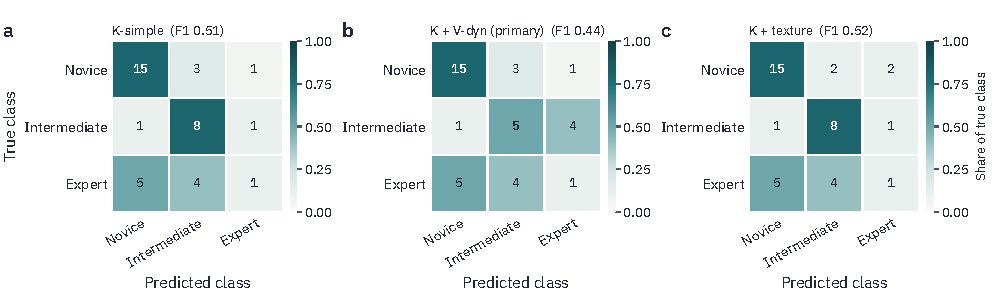
\includegraphics{fig4_confusion.pdf}
\caption{Pooled confusion matrices of (a) K-simple, (b) the primary multimodal model and (c) K-simple with motion texture. Numbers are trial counts; colour is the share of the true class.}
\label{fig:confusion}
\end{figure}

\begin{figure}[htbp]
\centering
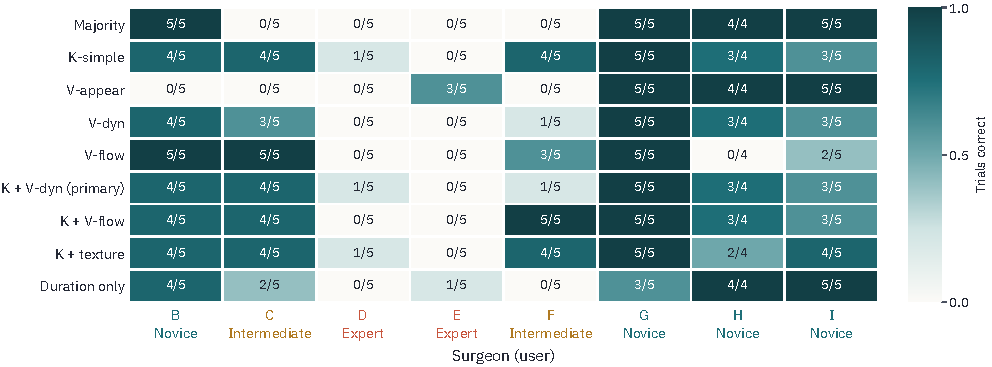
\includegraphics{fig5_users.pdf}
\caption{Correct trials per held-out surgeon for selected models. Each column is one LOUO fold; the label below gives the surgeon's skill level. Expert D and expert E are the dominant failure for every model except V-appear, which instead fails on novice B and both intermediates.}
\label{fig:users}
\end{figure}

Figure~\ref{fig:cases} shows the same pattern for single trials. The clearest successes are trials whose pace is typical of their class. Novice trial G001 lasts \CaseGZeroOneDur{}\,s and is labelled novice with probability \CaseGZeroOnePPred{}, and intermediate trial C004 lasts \CaseCZeroFourDur{}\,s and is labelled intermediate with probability \CaseCZeroFourPPred{}. The two experts fail in opposite directions, which is what a model that has learned one person rather than a class would do. When E is held out, the only training expert is D, whose trials last \DurRangeD{}\,s. E's trials last \DurRangeE{}\,s, so they probably look slow for an expert, and all five are labelled novice; E001 (\CaseEZeroOneDur{}\,s) receives a novice probability of \CaseEZeroOnePPred{} and an expert probability of only \CaseEZeroOnePTrue{}. When D is held out, the only training expert is E, so the fastest training trials belong to the intermediates (\DurRangeCF{}\,s), and four of D's five trials are labelled intermediate. This includes D005, the shortest trial in the dataset at \CaseDZeroFiveDur{}\,s, which receives an intermediate probability of \CaseDZeroFivePPred{} and an expert probability of \CaseDZeroFivePTrue{}. Not every error follows from duration. The last two trials of novice I are labelled intermediate with high confidence although both last about two minutes (I005, \CaseIZeroFiveDur{}\,s, intermediate probability \CaseIZeroFivePPred{}), so the model also responds to K-simple features other than the trial length.

\begin{figure}[htbp]
\centering
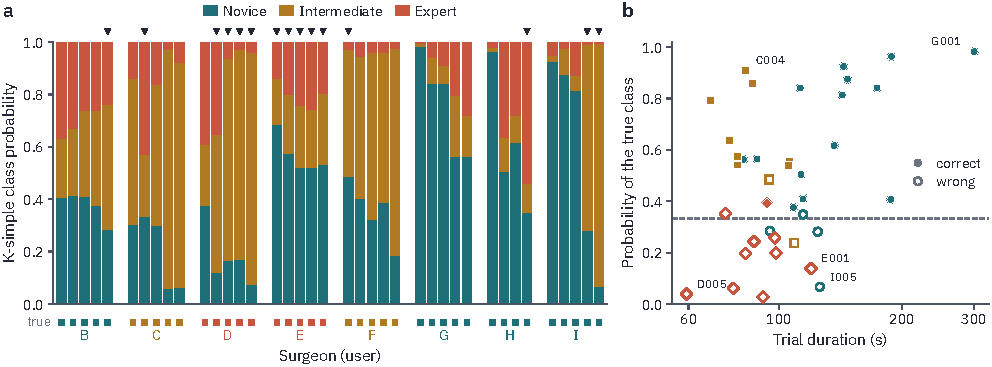
\includegraphics{fig7_cases.pdf}
\caption{Trial-level predictions of K-simple. (a) Class probabilities for every trial, grouped by held-out surgeon; squares below the bars give the true class and triangles mark wrong predictions. (b) Probability assigned to the true class against trial duration (log scale); filled markers are correct predictions, open markers are errors, and the dashed line is chance (1/3). The labelled trials are discussed in the text.}
\label{fig:cases}
\end{figure}


The pace audit shows how much of the kinematic signal is speed. A classifier on duration alone (C1) reaches macro-F1 \FCOne{}, well above the majority class, and the median absolute correlation of the K-simple features with log duration is \PaceKSimple{}. When every K-simple feature is residualised on log duration inside the training folds (C2), macro-F1 falls from \FMOne{} to \FCTwo{}, and the same happens with the texture block added (C2t, \FCTwoT{}). The skill information that K-simple transfers to new surgeons is therefore largely carried by how long the trial takes and by the quantities that scale with it (Figure~\ref{fig:audit}b). This is plausible for the novice versus trained distinction in a bench-top task, where trained surgeons are faster, but it is not a measure of quality and it explains why the expert class is missed.

\begin{figure}[htbp]
\centering
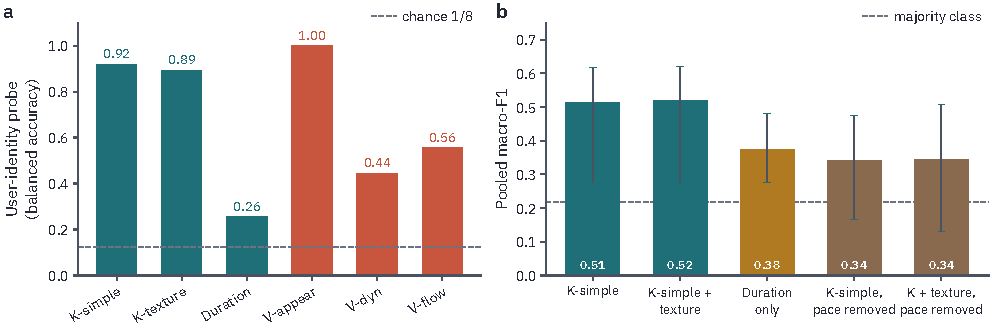
\includegraphics{fig6_audit.pdf}
\caption{Shortcut audit. (a) Balanced accuracy of an eight-way surgeon-identity probe on each feature block (stratified five-fold over trials); the dashed line is chance. (b) Macro-F1 of the kinematic models compared with a duration-only classifier and with the same kinematic features after removing their linear dependence on log duration inside each training fold.}
\label{fig:audit}
\end{figure}

The video results are explained by the same two mechanisms. V-appear identifies the surgeon perfectly (balanced accuracy \IdVAppear{}), yet as a skill classifier it reaches only \FMTwoA{}, and Figure~\ref{fig:users} shows the pattern expected of a block that recognises recording sessions: it is correct for all trials of the novices G, H and I and for three trials of expert E, but wrong for every trial of novice B and of both intermediates. The occasional success on expert E is therefore unlikely to reflect skill. V-dyn, designed to cancel static appearance, carries much less identity (\IdVDyn{}) but is strongly tied to pace: its median absolute correlation with log duration is \PaceVDyn{}, higher than that of K-simple. It thus adds a noisier copy of information the kinematic model already has. Late fusion with equal weights then hurts whenever the video classifier errs on a surgeon that kinematics gets right. The clearest case is intermediate F, for whom K-simple is correct on 4 of 5 trials and V-dyn on 1 of 5; after averaging, the fused model is correct on only \UFMThree{} (Figure~\ref{fig:users}). V-flow complements kinematics on F (fused \UFMThreeC{}) but fails completely on novice H, so its fusion again ends below kinematics alone.

The motion-texture improvement failed for a reason that can be seen in the features. The log dimensionless jerk of each instrument correlates with log duration at $|r| = \PaceKTextureMax{}$, which agrees with the known sensitivity of dimensionless jerk to movement duration \citep{hogan2009smoothness}, and the texture block identifies the surgeon almost as well as K-simple does (\IdKTexture{}). The ten texture features therefore largely duplicate the pace and identity information that K-simple already contains. Our block is also much smaller than the bank used by \citet{zia2018rmis}, who computed approximate entropy on every kinematic channel; we did not test the larger bank, because it was not part of the pre-declared protocol and choosing it after seeing these results would bias the comparison.

\subsection{Implementation and configuration details}

The inner LOUO selection chose strong regularisation in most folds ($C$ between 0.01 and 0.1 in seven of eight folds for K-simple), which is consistent with the small number of training surgeons. For V-appear the inner loop chose four principal components in six of eight folds. One inner fold was skipped in each of the outer folds C, D, E and F, as described in the protocol. Per-fold accuracy, averaged over surgeons, is \FoldAccMOne{} $\pm$ \FoldSdMOne{} (mean $\pm$ SD) for K-simple, and this per-fold spread is the reason we report pooled metrics with user-level intervals rather than a mean over folds. The code is organised as one module per stage (\texttt{data.py}, \texttt{features\_kin.py}, \texttt{features\_video.py}, \texttt{evaluate.py}), and \texttt{run\_all.py} reproduces every model, prediction file and statistic from the raw data in about five minutes; \texttt{make\_tables.py} and \texttt{make\_figures.py} regenerate the tables and figures of this report from the saved results without retraining.
